\section{Results}
When you start a new level, there will be an empty world as shown in \ref{fig:startup}. There will be connection points on both sides of the ravine. Depending on the level there could be more starting connection points. The user can start building a bridge by selecting a building block and a connection point. 
\begin{figure}[H]
    \centering
    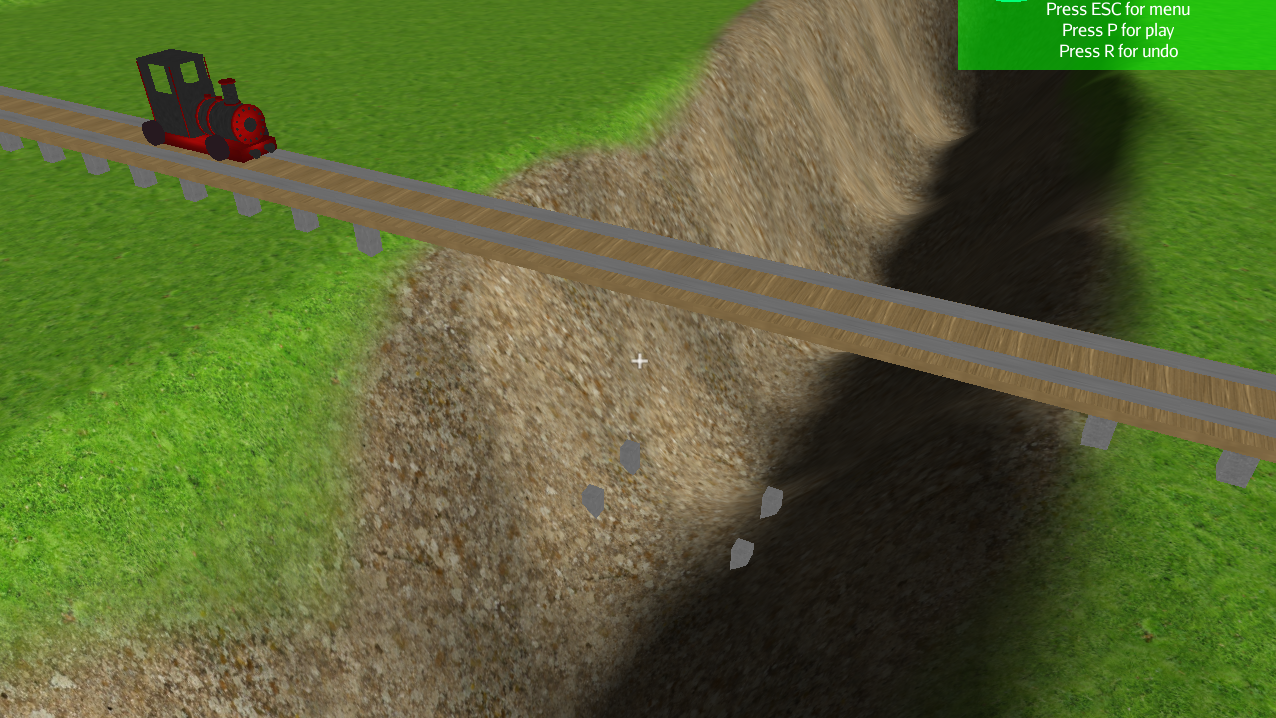
\includegraphics[width=0.8\textwidth]{screenshots/initial.png}
    \caption{Empty world}
    \label{fig:startup}
\end{figure}
After building a bridge the user can click on play, to start the simulation. The user cannot start the simulation if the 4 connection points are not connected. There has to be a connection between both sides of the ravine. A bridge built correctly is shown in \ref{fig:fullbridge}.
\begin{figure}[H]
    \centering
    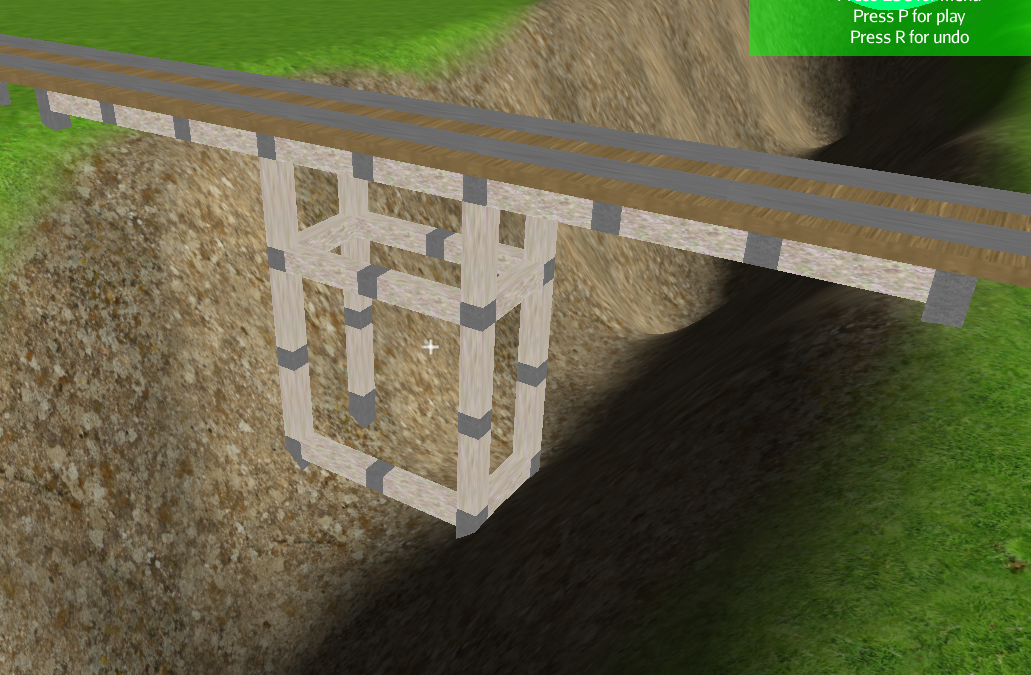
\includegraphics[width=0.8\textwidth]{screenshots/fullbridge.png}
    \caption{Bridge}
    \label{fig:fullbridge}
\end{figure}
When the user clicked on play and the bridge is built correctly, there will be a rail added automatically to the bridge. A train will ride over the bridge and the bridge will collapse or the train gets to the other side of the ravine safely as show in \ref{fig:full}
\begin{figure}[H]
    \centering
    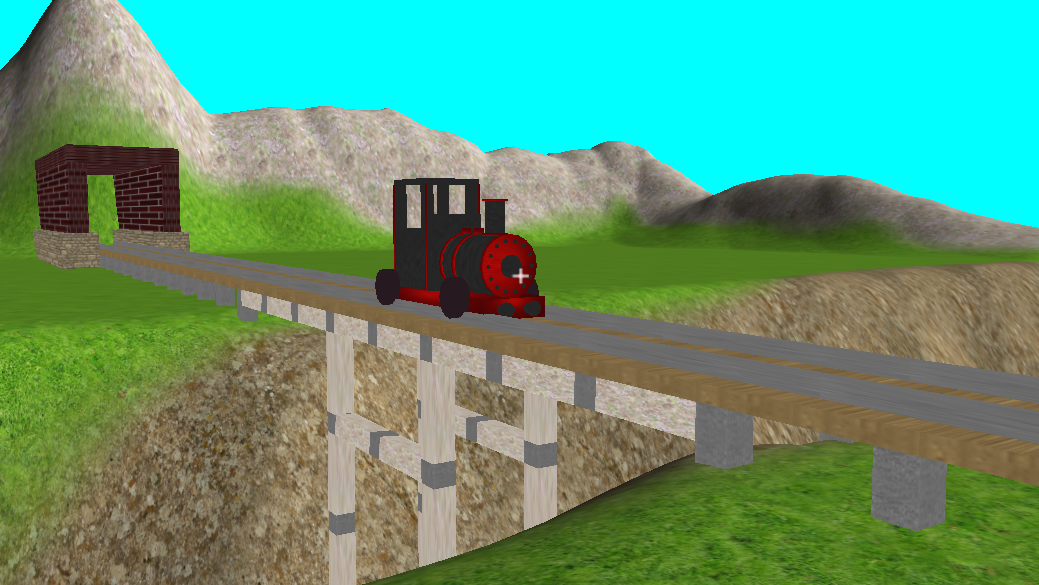
\includegraphics[width=0.8\textwidth]{screenshots/Drives.png}
    \caption{Succeed!}
    \label{fig:full}
\end{figure}